\documentclass{article}

\usepackage{csquotes}
% 使用中文CJK包
\usepackage{CJK}
% 图像插入宏包
\usepackage{graphicx}
% 自定义颜色支持
\usepackage[usenames,dvipsnames]{color}
% 长表格跨页支持
\usepackage{longtable}
% 代码高亮支持
\usepackage{listings}
% 算法伪代码包
\usepackage[ruled,vlined]{algorithm2e}
% 自定义标题格式
\usepackage{titlesec}
% 扩展tabular样式
\usepackage{array}
% 添加页眉页脚
\usepackage{fancyhdr}
% 虚拟正文测试
\usepackage{lipsum}
% 数学环境包
\usepackage{amsmath}
% 首行缩进
\usepackage{indentfirst}
% 树状结构图
\usepackage{tree-dvips}
% 脚注环境
\usepackage{footnote}
% 定制表格线
\usepackage{makecell}
% tikz绘图包
\usepackage{tikz}
% URL超链接
\usepackage[dvips, colorlinks, linkcolor=black]{hyperref}
% 断行URL超链接
\usepackage{breakurl}


% hyperref中文兼容
\pdfstringdefDisableCommands{
\let\CJK@XX\relax
\let\CJK@XXX\relax
\let\CJK@XXXp\relax
\let\CJK@XXXX\relax
\let\CJK@XXXXp\relax
}

\usetikzlibrary{positioning,shapes,shadows,arrows}


% 设置脚注在table中可用
\makesavenoteenv{table}

% 设置标题格式
%\titleformat{\chapter}{\raggedright\Huge\bfseries}{Chapter \thechapter}{1em}{}

% 设置默认字体族, 具体字体请查看texdoc psnfss2e

% 设置Roman字体为Palatino
\renewcommand{\rmdefault}{ppl} 
% 设置TypeWriter字体为Courier
\renewcommand{\ttdefault}{pcr} 

% 设置行距
\setlength{\parskip}{1ex}

% 定义需要的颜色

\definecolor{lightgray}{RGB}{230,230,230}
\definecolor{lightblue}{RGB}{224, 224, 255}
\definecolor{darkblue}{RGB}{192, 192, 255}
\definecolor{lightpink}{RGB}{255, 224, 224}
\definecolor{darkpink}{RGB}{255, 192, 192}
\definecolor{keywordyellow}{RGB}{255, 204, 0}
\definecolor{keywordred}{RGB}{194, 58, 0}
\definecolor{numbercolor}{RGB}{102, 51, 0}

% 设置代码风格

% 定义C语言代码风格
\lstdefinestyle{ccode}
{ 
    language=C, 
    numbers=left, 
    numberstyle=\color{numbercolor},
    basicstyle=\scriptsize\ttfamily\bfseries,
    keywordstyle=\color{blue}, 
    commentstyle=\color{PineGreen},
    stringstyle=\color{red}, 
    frame=shadowbox, 
    frameround=tttt,
    breaklines=true,
    backgroundcolor=\color{lightgray} }

% 定义汇编语言代码风格
\lstdefinestyle{acode}
{ 
    language=,
    morekeywords=[1]{mov, movl, movb, movw, orl, xorw, cli, cld, inb, testb, test, jnz, push, pop, jmp, call, lea, add, sub, ret, jle, outb, ljmp, lgdt, cmp, jne, popal, int},
    morekeywords=[2]{ax, bx, cx, dx, eax, ebx, ecx, edx, cr0, cr1, cr2, cr3, al, ds, es, ss, esp, ebp, esi, edi}, 
    morekeywords=[3]{data, text, bss},
    morekeywords=[4]{long, align, p2align, ascii, fill, globl, space, set, rept, byte, word},
    morecomment=[l]\#,
    numbers=left, 
    numberstyle=\color{numbercolor},
    basicstyle=\scriptsize\ttfamily\bfseries,
    keywordstyle=[1]\color{blue}, 
    keywordstyle=[2]\color{keywordyellow},
    keywordstyle=[3]\color{orange},
    keywordstyle=[4]\color{keywordred},
    commentstyle=\color{PineGreen},
    stringstyle=\color{red}, 
    frame=shadowbox, 
    frameround=tttt,
    breaklines=true,
    backgroundcolor=\color{lightgray} }

    
% 定义命令行输出风格
\lstdefinestyle{console}
{
    language=bash, 
    numbers=none, 
    frame=tRBl,
    basicstyle=\scriptsize\color{green}\ttfamily\bfseries,     
    backgroundcolor=\color{black}}


% 定义exercise输出风格
\lstdefinestyle{exercise}
{
    numbers=none, 
    frame=tRBl,
    breaklines=true,
    breakindent=0pt,
    framexleftmargin=1em,
    framexrightmargin=1em,
    framextopmargin=2ex,
    framexbottommargin=2ex,
    xleftmargin=0.05\linewidth,
    xrightmargin=0.05\linewidth,
    basicstyle=\scriptsize\ttfamily\mdseries,   
    moredelim=[is][\ttfamily\bfseries]{|}{|},
    framerule=0.8pt,
    rulecolor=\color{darkblue}, 
    backgroundcolor=\color{lightblue}}
    

% 定义challenge输出风格
\lstdefinestyle{challenge}
{
    numbers=none, 
    frame=tRBl,
    breaklines=true,
    breakindent=0pt,
    framexleftmargin=1em,
    framexrightmargin=1em,
    framextopmargin=2ex,
    framexbottommargin=2ex,
    xleftmargin=0.05\linewidth,
    xrightmargin=0.05\linewidth,
    basicstyle=\scriptsize\ttfamily\mdseries,   
    moredelim=[is][\ttfamily\bfseries]{|}{|},
    framerule=0.8pt,
    rulecolor=\color{darkpink}, 
    backgroundcolor=\color{lightpink}}
    


% 非常重要, listings关闭非ASCII字符兼容
\lstset{extendedchars=false}


% 定义问题的答案格式
\newcommand{\highlight}[1]{{\bfseries \color{red}  #1}}
% 定义函数名格式
\newcommand{\funcname}[1]{{\ttfamily \small #1}}




\pagestyle{fancy}
\begin{document}
\begin{CJK*}{UTF8}{gkai}

\lhead{操作系统实习报告}
\rhead{张弛, 00848231}
\title{操作系统JOS实习第三次报告}
\author{张弛 \hspace{1ex} 00848231, \\
        zhangchitc@gmail.com}

\maketitle
% 记得在文档末尾插入\clearpage
\tableofcontents
\newpage

\section{Introduction}

我在实验中主要参考了华中科技大学邵志远老师写的JOS实习指导,在邵老师的主页上\burl{http://grid.hust.edu.cn/zyshao/OSEngineering.htm} 可以找到。但是这次实验的指导远远不如lab1的指导详尽,所以我这里需要补充的内容会很多。

内联汇编请参考邵老师的第二章讲义,对于语法讲解的很详细。

\section{User Environments and Exception Handling}


\subsection{Environment State}

MIT的材料里对于\funcname{struct Env}的讲解很详细。其中唯一需要注意的就是\funcname{struct Trapframe}的理解,在这里还无法展开叙述。这个我们在后面具体编程的时候会提到。

\subsection{Allocating the Environments Array}


\begin{lstlisting}[style=exercise]
|Exercise 1|. Modify i386_vm_init() in kern/pmap.c to allocate and map the envs array. This array consists of exactly NENV instances of the Env structure allocated much like how you allocated the pages array. Also like the pages array, the memory backing envs should also be mapped user read-only at UENVS (defined in inc/memlayout.h) so user processes can read from this array.

You should run your code and make sure check_boot_pgdir() succeeds.
\end{lstlisting}

这个练习比较简单,有了前面设置pages数组的经验,对于envs的理解就很顺畅了。我们来看看具体的代码:

\begin{lstlisting}[style=ccode, title={\scriptsize \ttfamily \bfseries kern/pmap.c: i386\_vm\_init ()}]
	pages = boot_alloc (npage * sizeof (struct Page), PGSIZE);

	//////////////////////////////////////////////////////////////////////
	// Make 'envs' point to an array of size 'NENV' of 'struct Env'.
	// LAB 3: Your code here.
	
        envs = boot_alloc (NENV * sizeof (struct Env), PGSIZE);
\end{lstlisting}

分配了物理空间以后,再在虚拟地址空间为其创建映射:


\begin{lstlisting}[style=ccode, title={\scriptsize \ttfamily \bfseries kern/pmap.c: i386\_vm\_init ()}]
	//////////////////////////////////////////////////////////////////////
	// Map the 'envs' array read-only by the user at linear address UENVS
	// (ie. perm = PTE_U | PTE_P).
	// Permissions:
	//    - the new image at UENVS  -- kernel R, user R
	//    - envs itself -- kernel RW, user NONE
	// LAB 3: Your code here.
	//
        boot_map_segment (
            pgdir,
            UENVS,
            ROUNDUP (NENV * sizeof (struct Env), PGSIZE),
            PADDR ((uintptr_t) envs),
            PTE_U);
\end{lstlisting}


\subsection{Creating and Running Environments}

\begin{lstlisting}[style=exercise]
|Exercise 2|. In the file env.c, finish coding the following functions:

|env_init():|
        initialize all of the Env structures in the envs array and add them to the env_free_list.
|env_setup_vm():|
        allocate a page directory for a new environment and initialize the kernel portion of the new environment's address space.
|segment_alloc():|
        allocates and maps physical memory for an environment
|load_icode():|
        you will need to parse an ELF binary image, much like the boot loader already does, and load its contents into the user address space of a new environment.
|env_create():|
        allocate an environment with env_alloc and call load_icode load an ELF binary into it.
|env_run():|
        start a given environment running in user mode.

As you write these functions, you might find the new cprintf verb %e useful -- it prints a description corresponding to an error code. For example,

	r = -E_NO_MEM;
	panic("env_alloc: %e", r);
	
will panic with the message "env_alloc: out of memory".
\end{lstlisting}

\vspace{4em}

我们一个一个函数的来看把,首先是\funcname{env\_init()}:

\begin{lstlisting}[style=ccode, title={\scriptsize \ttfamily \bfseries kern/env.c: env\_init ()}]
void
env_init(void)
{
	int i;

	LIST_INIT(&env_free_list);
	for (i = NENV - 1; i >= 0; i--) {
		envs[i].env_id = 0;
                envs[i].env_status = ENV_FREE; 
		LIST_INSERT_HEAD(&env_free_list, &envs[i], env_link);
	}
}
\end{lstlisting}

没有什么好说的,类比pages对应的\funcname{page\_init()}写就行了。接下来看 \funcname{ env\_setup\_vm() }

\begin{lstlisting}[style=ccode, title={\scriptsize \ttfamily \bfseries kern/env.c: env\_setup\_vm ()}]
static int
env_setup_vm(struct Env *e)
{
	int i, r;
	struct Page *p = NULL;

	// Allocate a page for the page directory
	if ((r = page_alloc(&p)) < 0)
		return r;
		
        e->env_pgdir = page2kva (p);
        e->env_cr3 = page2pa (p);

        memmove (e->env_pgdir, boot_pgdir, PGSIZE);
        memset (e->env_pgdir, 0, PDX(UTOP) * sizeof (pde_t));
   
        p->pp_ref ++;
    
\end{lstlisting}

这里主要注意的是第14和15行代码。因为在UTOP之上的所有映射对于任何一个地址空间都是一样的(无论是对于内核地址空间还是对于任意一个用户地址空间而言),他们都和在lab2中对于内核地址空间设置的静态映射一样(静态映射就是没有实际分配物理页,即映射是通过\funcname{boot\_map\_segment()}而非\funcname{page\_insert()}),所以这里我们能直接拷贝系统页目录boot\_pgdir中的内容。

接下来看看函数\funcname{segment\_alloc()}

\begin{lstlisting}[style=ccode, title={\scriptsize \ttfamily \bfseries kern/env.c: segment\_alloc ()}]
static void
segment_alloc(struct Env *e, void *va, size_t len)
{
    va = ROUNDDOWN (va, PGSIZE);
    len = ROUNDUP (len, PGSIZE);

    struct Page *pp;
    int r;

    for (; len > 0; len -= PGSIZE, va += PGSIZE) {
        r = page_alloc (&pp);

        if (r != 0)
            panic ("segment_alloc: physical page allocation failed  %e", r);

        r = page_insert (e->env_pgdir, pp, va, PTE_U|PTE_W);

        if (r != 0)
            panic ("segment_alloc: page mapping failed  %e", r);
    } 
}
\end{lstlisting}

这个函数的作用是在e代表的用户虚拟地址空间中从va开始的地址分配出len长度的区域,准备写入数据。

有点类似lab2中的 \funcname{boot\_map\_segment()} ,但是他们是不一样的。 \funcname{boot\_map\_segment()} 的操作空间是内核虚拟地址空间boot\_pgdir。它提供的映射是静态映射,不涉及物理页的分配。而\funcname{segment\_alloc()} 则是要对实际的物理页面分配映射到当前用户的虚拟地址空间中。

弄清楚这两种映射机制的区别,上面的代码就很好理解了,看下一个函数\funcname{load\_icode()}


\begin{lstlisting}[style=ccode, title={\scriptsize \ttfamily \bfseries kern/env.c: load\_icode ()}]
static void
load_icode(struct Env *e, uint8_t *binary, size_t size)
{
    struct Elf *ELFHDR = (struct Elf*) binary;
    struct Proghdr *ph, *eph;

    // is this a valid ELF?
    if (ELFHDR->e_magic != ELF_MAGIC)
        panic ("load_icode: Not a valid ELF");

    ph = (struct Proghdr *) ((uint8_t *) ELFHDR + ELFHDR->e_phoff);
    eph = ph + ELFHDR->e_phnum;

    lcr3 (e->env_cr3);
    for (; ph < eph; ph++) {
        if (ph->p_type == ELF_PROG_LOAD) {
            segment_alloc (e, (void*) ph->p_va, ph->p_memsz);
            memset ((void *)ph->p_va, 0, ph->p_memsz);
            memmove ((void *)ph->p_va, binary + ph->p_offset, ph->p_filesz);
       }
    }
    lcr3 (boot_cr3);
    
    e->env_tf.tf_eip = ELFHDR->e_entry;

    segment_alloc (e, (void*) (USTACKTOP - PGSIZE), PGSIZE);
}
\end{lstlisting}

因为MIT的说明里提到过,因为JOS到现在为止还没有文件系统,所以为了测试我们能运行用户程序,现在的做法是将用户程序编译以后\highlight{和内核链接到一起}(即用户程序紧接着内核后面放置)。所以这个函数的作用就是将嵌入在内核中的用户程序取出释放到相应链接器指定好的用户虚拟空间里。这里的binary指针,就是用户程序在内核中的开始位置的虚拟地址。

按照注释的提示,我们可以参照boot/main.c来完成相应的载入,但是有几个地方需要注意

\begin{enumerate}
\item{对于用户程序ELF文件的每个程序头ph,ph$\rightarrow$p\_memsz和ph$\rightarrow$p\_filesz是两个概念,前者是该程序头应在\highlight{内存中占用的空间大小},而后者是实际该程序头\highlight{占用的文件大小}。他们俩的区别就是ELF文件中BSS节中那些没有被初始化的静态变量,这些变量不会被分配文件储存空间,但是在实际载入后,需要在内存中给与相应的空间,并且全部初始化为0。所以具体来讲,就是每个程序段ph,总共占用p\_memsz的内存,前面p\_filesz的空间从binary的对应内存复制过来,后面剩下的空间全部清0}
\item{ph$\rightarrow$p\_va是该程序段应该被放入的虚拟空间地址,但是注意,在这个时候,虚拟地址空间是\highlight{用户环境Env的虚拟地址空间}。可是,在进入 \funcname{load\_icode()} 时,是内核态进入的,所以虚拟地址空间还是内核的空间。我们要如何对用户的虚拟空间进行操作呢?看到第15行:

\begin{lstlisting}[style=ccode, firstnumber=15, title={\scriptsize \ttfamily \bfseries kern/env.c: load\_icode ()}]
    lcr3 (e->env_cr3);
\end{lstlisting}

这个语句在我们进入每个程序头进行具体设置时,将页表切换到用户虚拟地址空间。这样我们就可以方便的在后面使用memset和memmove等函数对一个虚拟地址进行相应的操作了。其中e$\rightarrow$env\_cr3的值是在前面的 \funcname{env\_setup\_vm()} 设置好的。

但是仍要小心的是,对于ELF载入完毕以后,我们就不需要对用户空间进行操作了,所以记得在22行重新切回到内核虚拟地址空间来。}
\item{注释中还提到了要对程序的入口地址作一定的设置,这里对应的操作是
\begin{lstlisting}[style=ccode, firstnumber=24, title={\scriptsize \ttfamily \bfseries kern/env.c: load\_icode ()}]
    e->env_tf.tf_eip = ELFHDR->e_entry;
\end{lstlisting}

这里涉及到对 struct Trapframe 结构的具体介绍,我们留到下一个函数说明 \funcname{env\_create()} 的时候进行详细介绍。
}
\end{enumerate}


\vspace{2em}

继续看下个函数\funcname{env\_create()}

\begin{lstlisting}[style=ccode, title={\scriptsize \ttfamily \bfseries kern/env.c: env\_create()}]
void
env_create(uint8_t *binary, size_t size)
{
    struct Env *e;
    int r;

    r = env_alloc (&e, 0);

    if (r < 0)
        panic ("env_create: %e", r);

    load_icode (e, binary, size);
}
\end{lstlisting}

到这个函数为止,系统就为一个用户程序的运行做好了一切准备,在这个函数中,接受内核传入的用户程序的所在地址binary(内核地址),然后为其创建用户进程空间,并且将其载入到相应的虚拟地址上。接下来的 \funcname{env\_run()}就可以开始真正的运行一个程序了。

这里调用了过程 \funcname{env\_alloc()} 来为用户进程分配一个struct Env,这个过程是JOS替我们写好的,但是还是有必要好好看看,便于我们对struct Env和struct Trapframe的理解。

MIT的资料中详细介绍了struct Env的结构:

\begin{lstlisting}[style=ccode, title={\scriptsize \ttfamily \bfseries inc/env.h}]
struct Env {
        struct Trapframe env_tf;        // Saved registers
        LIST_ENTRY(Env) env_link;       // Free list link pointers
        envid_t env_id;                 // Unique environment identifier
        envid_t env_parent_id;          // env_id of this env's parent
        unsigned env_status;            // Status of the environment
        uint32_t env_runs;              // Number of times environment has run

        // Address space
        pde_t *env_pgdir;               // Kernel virtual address of page dir
        physaddr_t env_cr3;             // Physical address of page dir
};
\end{lstlisting}

其中env\_tf的说明是保存了用户进程被切换出来时CPU的状态信息。我们去inc/trap.h中找寻其具体定义:

\begin{lstlisting}[style=ccode, title={\scriptsize \ttfamily \bfseries inc/trap.h}]
struct PushRegs {
	/* registers as pushed by pusha */
	uint32_t reg_edi;
	uint32_t reg_esi;
	uint32_t reg_ebp;
	uint32_t reg_oesp;		/* Useless */
	uint32_t reg_ebx;
	uint32_t reg_edx;
	uint32_t reg_ecx;
	uint32_t reg_eax;
} __attribute__((packed));

struct Trapframe {
	struct PushRegs tf_regs;
	uint16_t tf_es;
	uint16_t tf_padding1;
	uint16_t tf_ds;
	uint16_t tf_padding2;
	uint32_t tf_trapno;
	/* below here defined by x86 hardware */
	uint32_t tf_err;
	uintptr_t tf_eip;
	uint16_t tf_cs;
	uint16_t tf_padding3;
	uint32_t tf_eflags;
	/* below here only when crossing rings, such as from user to kernel */
	uintptr_t tf_esp;
	uint16_t tf_ss;
	uint16_t tf_padding4;
} __attribute__((packed));
\end{lstlisting}

其他的都很好理解,某些padding开头的变量是为了让数据补齐4Byte。

我们看到,Trapframe保存的都是一些系统关键的寄存器。这里我们只需要特别关注4个寄存器,涉及到程序执行的控制流问题:

\begin{itemize}
\item{EFLAGS: 状态寄存器,这个我们暂时用不到}
\item{EIP:Instruction Pointer,当前执行的汇编指令的地址}
\item{ESP:当前的栈顶地址}
\item{EBP:辅助用,当前过程的帧在栈中的开始地址(高地址)即EBP到EIP中就是此过程的帧}
\end{itemize}

其中EBP由程序自行操作,而其他三者都会被在执行汇编指令时被改变。ESP就不说了,push和pop指令都是以ESP指针为操作目标的。至于EIP,在lab1中的运行栈那一节,我们看到了C程序编译后压栈的具体信息,其中就可以看到EIP。现在我们可以来看看在程序调用call时具体是如何修改EIP的。通过查询{\ttfamily \bfseries IA-32 Intel Architecture Software Developer's Manuals } 中的  {\ttfamily \bfseries Volume 2A: Instruction Set Reference, A-M } 中的CALL指令,我们可以看到其详细的执行流程:


\begin{algorithm}[htp]
\dontprintsemicolon
\Begin{
$tempEIP \longleftarrow EIP + DEST;$\;
Push($EIP$);\;
$EIP \longleftarrow tempEIP;$\;
}
\caption{CALL - Call Procedure}
\end{algorithm}

这个是我个人简化后最关键的部分,实际上指令的流程涉及到32位、64位、访问权限、以及长跳转和短跳转的各种问题,不过那不是我们关心的。我们只需要知道\highlight{它对EIP和ESP作了什么
}就好了。

从上面简单的三条语句我们可以知道,在进入新的过程体之前,老的EIP就被系统压入了堆栈以便后面返回时使用,然后将新的执行地址放入了EIP。CALL执行完以后,ESP和EIP都发生了改变。

同样的有调用就有返回,我们去看看RET指令的详细手册:

\begin{algorithm}[htp]
\dontprintsemicolon
\Begin{
$EIP \longleftarrow$ Pop();\;
}
\caption{RET - Return from Procedure}
\end{algorithm}

看着很简单,如果涉及保护模式和实模式的切换,那么还有相应段寄存器CS的保存切换问题,在IRET中我们就可以看到相应的逻辑,现在我们先可以不管。

\vspace{4em}

好了,看完Trapframe的内部结构和关键寄存器以后,我们回到Trapframe的讨论。既然这里保存了程序执行所需要的状态,那么刚才在 \funcname{load\_icode()} 中是如何设置的呢,在 \funcname {env\_create() }调用\funcname{load\_icode()}之前分配用户环境 \funcname{env\_alloc()} 。我们进这里看看:

\begin{lstlisting}[style=ccode, title={\scriptsize \ttfamily \bfseries kern/env.c: env\_alloc()}]
int
env_alloc(struct Env **newenv_store, envid_t parent_id)
{
	int32_t generation;
	int r;
	struct Env *e;

	if (!(e = LIST_FIRST(&env_free_list)))
		return -E_NO_FREE_ENV;

	// Allocate and set up the page directory for this environment.
	if ((r = env_setup_vm(e)) < 0)
		return r;

	// Generate an env_id for this environment.
	generation = (e->env_id + (1 << ENVGENSHIFT)) & ~(NENV - 1);
	if (generation <= 0)	// Don't create a negative env_id.
		generation = 1 << ENVGENSHIFT;
	e->env_id = generation | (e - envs);
	
	// Set the basic status variables.
	e->env_parent_id = parent_id;
	e->env_status = ENV_RUNNABLE;
	e->env_runs = 0;

	// Clear out all the saved register state,
	// to prevent the register values
	// of a prior environment inhabiting this Env structure
	// from "leaking" into our new environment.
	memset(&e->env_tf, 0, sizeof(e->env_tf));

	// Set up appropriate initial values for the segment registers.
	// GD_UD is the user data segment selector in the GDT, and 
	// GD_UT is the user text segment selector (see inc/memlayout.h).
	// The low 2 bits of each segment register contains the
	// Requestor Privilege Level (RPL); 3 means user mode.
	e->env_tf.tf_ds = GD_UD | 3;
	e->env_tf.tf_es = GD_UD | 3;
	e->env_tf.tf_ss = GD_UD | 3;
	e->env_tf.tf_esp = USTACKTOP;
	e->env_tf.tf_cs = GD_UT | 3;
	// You will set e->env_tf.tf_eip later.

	// commit the allocation
	LIST_REMOVE(e, env_link);
	*newenv_store = e;

	cprintf("[%08x] new env %08x\n", curenv ? curenv->env_id : 0, e->env_id);
	return 0;
}
\end{lstlisting}

我们只需要关注从26行开始以后的内容,这里开始对e$\rightarrow$env\_tf进行设置。有几个关键点:

\begin{itemize}
\item{tf\_esp:初始化为USTACKTOP,表示当前用户栈为空}
\item{tf\_cs: 初始化为user text segment selector,权限为用户可访问}
\item{tf\_eip: 这里没有设置,但是注释告诉我们了该由我们设置,很显然,这里eip的值就是我们在 \funcname{load\_icode()} 里应该设置的用户程序入口地址}
\end{itemize}

这样梳理一遍以后,我们就可以对 \funcname{load\_icode()} 里那行设置入口地址代码完全理解了。

看到最后一个要完成的过程 \funcname{env\_run()}


\begin{lstlisting}[style=ccode, title={\scriptsize \ttfamily \bfseries kern/env.c: env\_run()}]
void
env_run(struct Env *e)
{
    if (curenv != e) {
        curenv = e;
        curenv->env_runs ++;
        lcr3 (curenv->env_cr3);
    }

    env_pop_tf (&curenv->env_tf);

	panic("env_run not yet implemented");
}
\end{lstlisting}

这里的一个问题就是处理重复切换到当前用户环境的判断,只有是切换到一个新的用户环境时,才需要启用新的用户页面。这个过程里最主要的任务是理解 \funcname{env\_pop\_tf()} ,这个过程是真正负责切换到用户程序的过程:


\begin{lstlisting}[style=ccode, title={\scriptsize \ttfamily \bfseries kern/env.c: env\_pop\_tf()}]
void
env_pop_tf(struct Trapframe *tf)
{
	__asm __volatile("movl %0,%%esp\n"
		"\tpopal\n"
		"\tpopl %%es\n"
		"\tpopl %%ds\n"
		"\taddl $0x8,%%esp\n" /* skip tf_trapno and tf_errcode */
		"\tiret"
		: : "g" (tf) : "memory");
	panic("iret failed");  /* mostly to placate the compiler */
}
\end{lstlisting}

我们来尝试理解这段内联汇编:

\begin{lstlisting}[style=acode, firstnumber=4]
        movl %0,%%esp
\end{lstlisting}

这里出现了占位符\%0,通过后面的参数可以看到这里的占位符代表的是memory中的变量tf,即Trapframe的指针地址。这里把它传给esp是什么意思?看到后面的各种pop命令,就可以知道,这里的想法是把Trapframe看作一个存储了很多内容的栈,然后利用pop命令一个一个输出到我们想要重置的寄存器里。因为我们知道弹栈的时候栈指针是不断加的过程(栈的生长是栈指针不断减),所以将ESP设置为Trapframe所在内存的首地址,就可以以内存中的排布顺序释放出所有的内容了。非常的巧妙!

\begin{lstlisting}[style=acode, firstnumber=5]
        popal
\end{lstlisting}

通过查询手册,可以得到popal的执行明细:

\begin{algorithm}[htp]
\dontprintsemicolon
\Begin{
$EDI \longleftarrow$ Pop();\;
$ESI \longleftarrow$ Pop();\;
$EBP \longleftarrow$ Pop();\;
$ESP \longleftarrow ESP + 4$ ;(* Skip next 4 bytes of stack *)\;
$EBX \longleftarrow$ Pop();\;
$EDX \longleftarrow$ Pop();\;
$ECX \longleftarrow$ Pop();\;
$EAX \longleftarrow$ Pop();\;
}
\caption{POPA - Pop All General Purpose Registers}
\end{algorithm}

第一句就输出了这么多寄存器,这里每一次Pop (),就是从ESP指向的Trapframe里拿出4个Byte,我们来看看Trapframe的前8个DWORD是什么:

\begin{lstlisting}[style=ccode, title={\scriptsize \ttfamily \bfseries inc/trap.h}]
struct PushRegs {
	/* registers as pushed by pusha */
	uint32_t reg_edi;
	uint32_t reg_esi;
	uint32_t reg_ebp;
	uint32_t reg_oesp;		/* Useless */
	uint32_t reg_ebx;
	uint32_t reg_edx;
	uint32_t reg_ecx;
	uint32_t reg_eax;
} __attribute__((packed));

struct Trapframe {
	struct PushRegs tf_regs;
	uint16_t tf_es;
	uint16_t tf_padding1;
	uint16_t tf_ds;
	uint16_t tf_padding2;
	uint32_t tf_trapno;
	/* below here defined by x86 hardware */
	uint32_t tf_err;
	uintptr_t tf_eip;
	uint16_t tf_cs;
	uint16_t tf_padding3;
	uint32_t tf_eflags;
	/* below here only when crossing rings, such as from user to kernel */
	uintptr_t tf_esp;
	uint16_t tf_ss;
	uint16_t tf_padding4;
} __attribute__((packed));
\end{lstlisting}

可以看到前8个DWORD为一个struct PushRegs,\highlight{这里面的定义顺序和popal里设置的顺序是完全对应的!}可见PushRegs的定义也是经过了缜密的思考的,非常的巧妙,利用一句汇编指令就完成了这么多寄存器的设置。

后面几句汇编代码就很好理解了,直到这句:

\begin{lstlisting}[style=acode, firstnumber=5]
        iret
\end{lstlisting}

再次求助INTEL的指令手册,可以看到IRET和RET的不同:

\begin{algorithm}[htp]
\dontprintsemicolon
\Begin{
$EIP \longleftarrow$ Pop();\;
$CS \longleftarrow$ Pop();\;
$FLAGS \longleftarrow$ Pop();\;
}
\caption{IRET - Interrupt Return}
\end{algorithm}

因为IRET涉及到中断返回的各种控制,所以在保护模式以及实模式切换中会涉及段寄存器切换以及访问控制的问题,实际的控制流非常非常非常复杂,有兴趣的同学可以参考手册里的详细说明。

这个时候执行的IRET语句,会把Trapframe里的下面三个成员放入相应的寄存器

\begin{lstlisting}[style=ccode, numbers=none]
	uintptr_t tf_eip;
	uint16_t tf_cs;
	uint16_t tf_padding3;
	uint32_t tf_eflags;
\end{lstlisting}

这些成员我们在\funcname{env\_alloc()} 以及\funcname{load\_icode()}中都设置好了,其中EIP为用户程序入口地址,CS为用户程序代码段段基址。

那么执行完这条语句以后,CPU再往下执行的第一条语句,应该就是用户程序的第一条指令了。

所以说\funcname{env\_run()}和 \funcname{env\_pop\_tf()}都是没有返回的。

\vspace{2em}

\hrule

\vspace{2em}

到这里,我们的Exercise 2就算做完了,但是编译启动JOS发现它给出了Triple fault的错误信息。在MIT的课程材料上解释了这样的原因。是因为我们没有对中断表进行相应的设置,以至于用户程序在调用系统终端输出字符时产生了错误。但是我们需要认为的确认一下是否真的错误是由中断而不是其他设置造成的,所以我们启动GDB调试,选择在\funcname{env\_pop\_tf()}函数停下:

\begin{lstlisting}[style=console]
The target architecture is assumed to be i8086
[f000:fff0]    0xffff0:	ljmp   $0xf000,$0xe05b
0x0000fff0 in ?? ()
+ symbol-file obj/kern/kernel
(gdb) b env_pop_tf
Breakpoint 1 at 0xf0103128: file kern/env.c, line 523.
(gdb) c
Continuing.
The target architecture is assumed to be i386
=> 0xf0103128 <env_pop_tf>:	push   %ebp

Breakpoint 1, env_pop_tf (tf=0xf01af000) at kern/env.c:523
523	{
(gdb) 
\end{lstlisting}

从这里开始单步跟踪,在IRET指令之前停下来,我们在这里查看寄存器的信息看是否都被设置好了:

\begin{lstlisting}[style=console]
(gdb) next
=> 0xf010312e <env_pop_tf+6>:	mov    0x8(%ebp),%esp
525		__asm __volatile("movl %0,%%esp\n"
(gdb) si
=> 0xf0103131 <env_pop_tf+9>:	popa   
0xf0103131	525		__asm __volatile("movl %0,%%esp\n"
(gdb) si
=> 0xf0103132 <env_pop_tf+10>:	pop    %es
0xf0103132 in env_pop_tf (tf=???) at kern/env.c:525
525		__asm __volatile("movl %0,%%esp\n"
(gdb) si
=> 0xf0103133 <env_pop_tf+11>:	pop    %ds
0xf0103133	525		__asm __volatile("movl %0,%%esp\n"
(gdb) si
=> 0xf0103134 <env_pop_tf+12>:	add    $0x8,%esp
0xf0103134	525		__asm __volatile("movl %0,%%esp\n"
(gdb) si
=> 0xf0103137 <env_pop_tf+15>:	iret   
0xf0103137	525		__asm __volatile("movl %0,%%esp\n"
(gdb) info registers 
eax            0x0	0
ecx            0x0	0
edx            0x0	0
ebx            0x0	0
esp            0xf01af030	0xf01af030
ebp            0x0	0x0
esi            0x0	0
edi            0x0	0
eip            0xf0103137	0xf0103137 <env_pop_tf+15>
eflags         0x96	[ PF AF SF ]
cs             0x8	8
ss             0x10	16
ds             0x23	35
es             0x23	35
fs             0x23	35
gs             0x23	35
(gdb) 
\end{lstlisting}

从EAX、ECX等寄存器中看到都被清0了,这个和我们在\funcname{env\_alloc()}中看到的设置是一致的,但是在IRET执行之前CS和EIP两个寄存器都还看不到,不过没有关系,我们知道栈顶的接下来三个DWORD分别为EIP、CS和EFLAGS,我们查看一下栈顶的这三个DWORD:

\begin{lstlisting}[style=console]
(gdb) x/3x 0xf01af030
0xf01af030:	0x00800020	0x0000001b	0x00000000
(gdb) 
\end{lstlisting}

可以看到EIP的值为0x00800020即用户程序的入口地址,我们可以打开user/user.ld文件查看一下:

\begin{lstlisting}[style=ccode, language=make, firstnumber=4, title={\scriptsize \ttfamily \bfseries user/user.ld}]
OUTPUT_FORMAT("elf32-i386", "elf32-i386", "elf32-i386")
OUTPUT_ARCH(i386)
ENTRY(_start)

SECTIONS
{
	/* Load programs at this address: "." means the current address */
	. = 0x800020;

	.text : {
		*(.text .stub .text.* .gnu.linkonce.t.*)
	}
\end{lstlisting}

可以看到第11行链接器对于程序入口地址的设置,和我们看到的调试结果是符合的。这就说明我们正确的将入口地址加载进来了,接下来我们看看是否正确载入了用户程序的ELF文件:


\begin{lstlisting}[style=console]
(gdb) si
=> 0x800020:	cmp    $0xeebfe000,%esp
0x00800020 in ?? ()
(gdb) x/6i 0x800020
=> 0x800020:	cmp    $0xeebfe000,%esp
   0x800026:	jne    0x80002c
   0x800028:	push   $0x0
   0x80002a:	push   $0x0
   0x80002c:	call   0x800060
   0x800031:	jmp    0x800031
(gdb) 
\end{lstlisting}

实际的用户程序hello的汇编代码可以在obj/user/hello.asm中找到:

\begin{lstlisting}[style=acode, firstnumber=5, title={\scriptsize \ttfamily \bfseries obj/user/hello.asm}]
Disassembly of section .text:

00800020 <_start>:
// starts us running when we are initially loaded into a new environment.
.text
.globl _start
_start:
	// See if we were started with arguments on the stack
	cmpl $USTACKTOP, %esp
  800020:	81 fc 00 e0 bf ee    	cmp    $0xeebfe000,%esp
	jne args_exist
  800026:	75 04                	jne    80002c <args_exist>

	// If not, push dummy argc/argv arguments.
	// This happens when we are loaded by the kernel,
	// because the kernel does not know about passing arguments.
	pushl $0
  800028:	6a 00                	push   $0x0
	pushl $0
  80002a:	6a 00                	push   $0x0

0080002c <args_exist>:

args_exist:
	call libmain
  80002c:	e8 2f 00 00 00       	call   800060 <libmain>
1:	jmp 1b
  800031:	eb fe                	jmp    800031 <args_exist+0x5>
	...
\end{lstlisting}

可以看到和输出是一致的,从这里可以知道我们的\funcname{load\_icode()} 的载入是正常工作的。

我们找到MIT教材中提到的\funcname{sys\_cputs()}函数中的中断指令在用户程序中的位置:

\begin{lstlisting}[style=acode, firstnumber=2074, title={\scriptsize \ttfamily \bfseries obj/user/hello.asm}]
void
sys_cputs(const char *s, size_t len)
{
  800d3c:	55                   	push   %ebp
  800d3d:	89 e5                	mov    %esp,%ebp
  800d3f:	83 ec 0c             	sub    $0xc,%esp
  800d42:	89 1c 24             	mov    %ebx,(%esp)
  800d45:	89 74 24 04          	mov    %esi,0x4(%esp)
  800d49:	89 7c 24 08          	mov    %edi,0x8(%esp)
	// 
	// The last clause tells the assembler that this can
	// potentially change the condition codes and arbitrary
	// memory locations.

	asm volatile("int %1\n"
  800d4d:	b8 00 00 00 00       	mov    $0x0,%eax
  800d52:	8b 4d 0c             	mov    0xc(%ebp),%ecx
  800d55:	8b 55 08             	mov    0x8(%ebp),%edx
  800d58:	89 c3                	mov    %eax,%ebx
  800d5a:	89 c7                	mov    %eax,%edi
  800d5c:	89 c6                	mov    %eax,%esi
  800d5e:	cd 30                	int    $0x30

void
sys_cputs(const char *s, size_t len)
{
	syscall(SYS_cputs, 0, (uint32_t)s, len, 0, 0, 0);
}
  800d60:	8b 1c 24             	mov    (%esp),%ebx
  800d63:	8b 74 24 04          	mov    0x4(%esp),%esi
  800d67:	8b 7c 24 08          	mov    0x8(%esp),%edi
  800d6b:	89 ec                	mov    %ebp,%esp
  800d6d:	5d                   	pop    %ebp
  800d6e:	c3                   	ret    
\end{lstlisting}

可以看到中断调用的地址为0x800d5e,我们尝试着在这里设下断点,看JOS能否运行到这里:

\begin{lstlisting}[style=console]
(gdb) b *0x800d5e
Breakpoint 2 at 0x800d5e
(gdb) c
Continuing.
=> 0x800d5e:	int    $0x30

Breakpoint 2, 0x00800d5e in ?? ()
(gdb) si
=> 0x800d5e:	int    $0x30

Breakpoint 2, 0x00800d5e in ?? ()
(gdb) 
\end{lstlisting}

可以看到JOS成功运行到了该断点,再执行一条指令,EIP没有发生变化,这个时候看QEMU的输出信息,发现已经产生Triple fault:


\begin{lstlisting}[style=console]
zhangchi@zhangchi-vostro1400:~/lab$ make qemu-gdb
sed "s/localhost:1234/localhost:26000/" < .gdbinit.tmpl > .gdbinit
***
*** Now run 'gdb'.
***
qemu -hda obj/kern/kernel.img -serial mon:stdio -S -gdb tcp::26000
6828 decimal is 15254 octal!
Hooray! Passed all test cases for stdlib!!
Physical memory: 66556K available, base = 640K, extended = 65532K
check_page_alloc() succeeded!
page_check() succeeded!
check_boot_pgdir() succeeded!
[00000000] new env 00001000
EAX=00000000 EBX=00000000 ECX=0000000d EDX=eebfde88
ESI=00000000 EDI=00000000 EBP=eebfde60 ESP=eebfde54
EIP=00800d5e EFL=00000092 [--S-A--] CPL=3 II=0 A20=1 SMM=0 HLT=0
ES =0023 00000000 ffffffff 00cff300 DPL=3 DS   [-WA]
CS =001b 00000000 ffffffff 00cffa00 DPL=3 CS32 [-R-]
SS =0023 00000000 ffffffff 00cff300 DPL=3 DS   [-WA]
DS =0023 00000000 ffffffff 00cff300 DPL=3 DS   [-WA]
FS =0023 00000000 ffffffff 00cff300 DPL=3 DS   [-WA]
GS =0023 00000000 ffffffff 00cff300 DPL=3 DS   [-WA]
LDT=0000 00000000 00000000 00008200 DPL=0 LDT
TR =0028 f017c8e0 00000068 f0408917 DPL=0 TSS32-avl
GDT=     f011a320 0000002f
IDT=     f017c0e0 000007ff
CR0=80050033 CR2=00000000 CR3=0005c000 CR4=00000000
DR0=00000000 DR1=00000000 DR2=00000000 DR3=00000000 
DR6=ffff0ff0 DR7=00000400
Triple fault.  Halting for inspection via QEMU monitor.

\end{lstlisting}

所以到目前为止,我们写出的JOS的运行一切正常。


\subsection{Handling Interrupts and Exceptions}

\begin{lstlisting}[style=exercise]
|Exercise 3|. Read Chapter 9, Exceptions and Interrupts in the 80386 Programmer's Manual (or Chapter 5 of the IA-32 Developer's Manual), if you haven't already.
\end{lstlisting}

一定要读!尤其是 {\ttfamily \bfseries  Chapter 9, Exceptions and Interrupts } ,因为IA-32的开发手册实在是太长没法看,但是前面这个HTML的说明不长不短,刚好能大致完整的介绍一下中断的机制。

在{\ttfamily \bfseries 9.5 IDT Descriptors} 中提到了IDT中一共有三种类型的门描述符

\begin{itemize}
\item{Task gates}
\item{Interrupt gates}
\item{Trap gates}
\end{itemize}

后来我在查找资料时在IA32-3A.pdf里看到了x86中关于门描述符的综合介绍(详见{\ttfamily \bfseries 4.8.2 Gate Descriptors}),发现还有一个Call gates,然后我就晕了,不知道这4种门都是干什么的,然后为什么IDT只有其中三种。

尽管在{\ttfamily \bfseries 9.6 Interrupt Tasks and Interrupt Procedures} 中稍微解释了一下,但是我觉得它没有讲清楚\highlight{为什么要区别开来这四种门,它们各自的不同分别对应什么样的应用场景等等}。我找到了一个中文版的说明:\burl{http://www.mouseos.com/arch/gate_descriptor.html} ,比前面那个网页版要详细一点,但是仍没有说到点子上。后来我终于找到StackOverflow上一个相关的问题,我觉得讲的很好:\burl{http://stackoverflow.com/questions/3425085/ the-difference-between-call-gate-interrupt-gate-trap-gate}。这里我就按照我的理解把上面的资料总结一下:

首先复习一下预备知识,通用寄存器EFLAGS保存的是CPU的执行状态和控制信息,如下图,其中我们只需要关注两个寄存器:\highlight{IF和TF}。


\begin{figure}[htp]
\centering
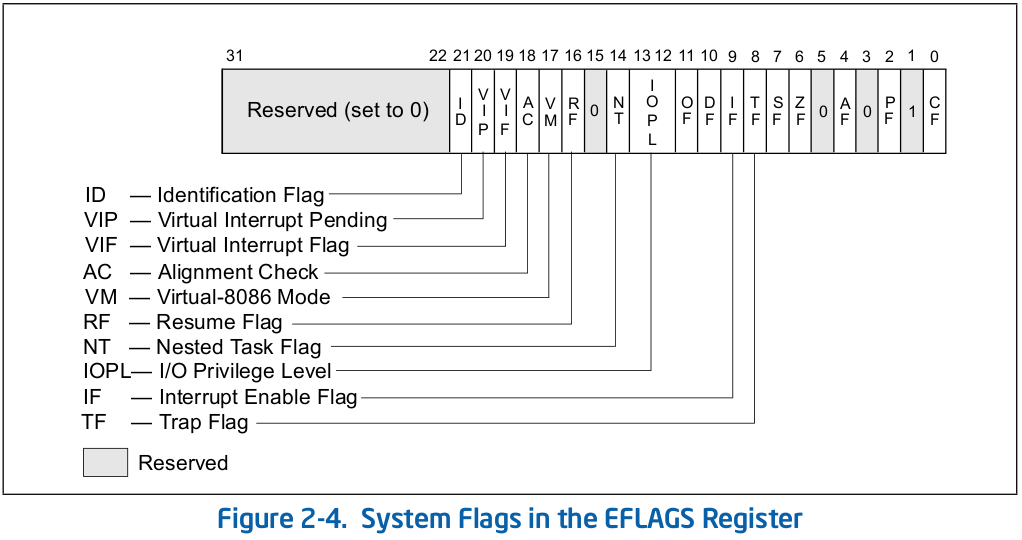
\includegraphics[scale=0.30]{/home/zhangchi/lab/report/EFLAGS.png}
\end{figure}



\begin{description}
\item[TF(Trap Flag)] :\\
跟踪标志。置1 则开启单步执行调试模式,置0 则关闭。在单步执行模式下,处理器在每条指令后产生一个调试异常,这样在每条指令执行后都可以查看执行程序的状态。
\item[IF (Interrupt enable)] :\\
中断许可标志。控制处理器对可屏蔽硬件中断请求的响应。置1 则开启可屏蔽硬件中断响应,置0 则关闭可屏蔽硬件中断响应。IF 标志不影响异常和不可屏蔽中断(NMI)的产生。
\end{description}


\vspace{1em}

\hrule

\vspace{1em}

门用来实现从一段代码跳转到另一段代码(可能在不同的代码段,不同特权级)时的保护机制问题。

其中\highlight{Interrupt gate和trap gate和另外两个的区别}是,他们用来专门处理处理器异常或者中断(Exception or interrupt),而另外两种一般处理用户的软件切换。


\begin{description}
\item[Interrupt gate 和 Trap gate的区别]: \\
我们可以看到这两者的描述符基本没有区别,而实际上它们的执行工作也基本类似,除了一点!就是\highlight{Interrupt gate会修改IF},会对中断响应屏蔽,即不再响应接下来的中断了

这个不同在处理什么情况时候会导致差别呢?上面链接中的网友提供了一个很好的实例,比如操作系统捕获了一个硬件中断正在处理,又来了另一个。如果用trap gate,那么第一个处理就被打断了,这样会造成数据崩溃。所以必须屏蔽掉第二个处理。这样的话可以使一次硬件操作成为\highlight{原子操作},保证处理的正确和完整。(当然,如果是NMI,那就另说了)


还有一个是断点异常的处理,这个中断必须暴露给用户程序进行调用。但是又要区别于中断,所以使用trap gate来处理。所以一般情况下,interrupt gate用于处理意外发生的错误,而trap gate用来处理人为制造的软件中断比如page fault、调试中断等等

\item[Call gate 和 Task gate的区别]: \\
首先x86中引入了Task的概念,具体请看IA32-3A.pdf的 {\ttfamily \bfseries CHAPTER 6 TASK MANAGEMENT } 一章,简单来说,task就是一个具体的可运行的单位,可以运行,挂起,重启等等,然后在这个单位上可以保存其状态到TSS(Task-state segment)去。我们可以通过一个CALL或者JMP指令来具体的调用一个task程序。

call gate和task gate都可以用来切换到一个task,\highlight{但是task gate的寻址需要经过一个TSS找到code selector}(具体见task gate descriptor)。当然这样显然比call gate麻烦,但是这样带来的好处是:

\begin{itemize}
\item{切换到时候原来task的上下文环境被自动保存(TSS)}
\item{如果使用task gate来处理中断例程,那么可以使程序和其他例程分开,使其具有独立的地址空间比如页表等等}
\end{itemize}

\end{description}

x86手册第一章有幅图能大致总结一下以上四种切换机制的具体细节:


\begin{figure}[htp]
\centering
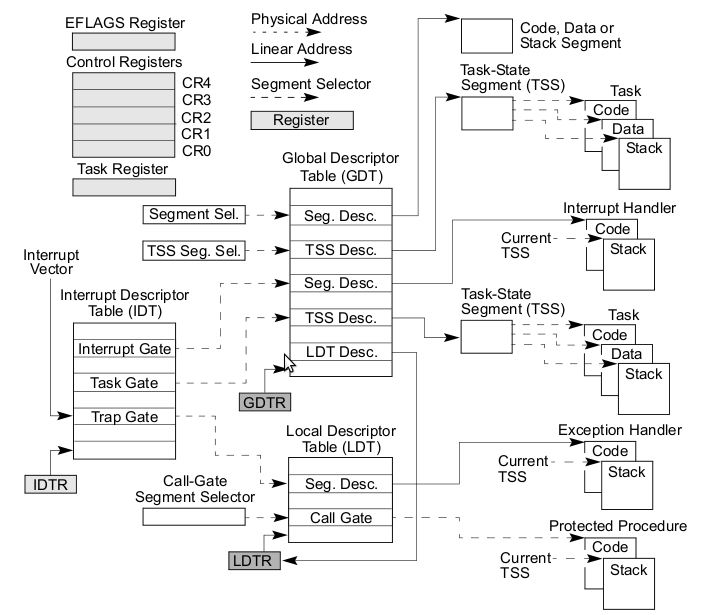
\includegraphics[scale=0.40]{/home/zhangchi/lab/report/IDT.png}
\end{figure}

\subsection{Basics of Protected Control Transfer}

这里开始提到IDT和TSS的具体构造,这里我主要想谈一谈TSS。

在IA32-3A.pdf的{\ttfamily \bfseries 6.2.1 Task-State Segment (TSS) } 有对其的详细描述,简而言之,为了能保存和恢复一个task的执行状态而引入了TSS的概念。TSS描述了一个task在执行中的状态信息。

但是我看到TSS的就想起了前面的struct Env结构,这两个东西不同样都是保存状态信息的么,有什么区别?

Env对应的是一个用户进程的状态,这里的进程是一个抽象程度较高的概念,而不仅仅是一段程序代码而已。它有独立的PCB,地址空间等等。所以对比struct Env和struct Taskstate的详细结构就可以知道,Env中有 env\_pgdir 和 env\_cr3 这种页表相关的成员,表示它不仅要保存CPU的即时运行状态,还要保存其空间页表的信息。

相比之下,TSS对应的则不是进程,而是比较底层的概念,是一段汇编代码中的过程。它比struct Env多出的像ESP0,SS0,ESP1,SS1这样的结构,重在描述代码切换之间权限的转换。

\highlight{综上,TSS侧重权限,主要用于保护机制,而Env则主要用于保持用户进程的独立}。两者适用的对象不同,目的和侧重点更不同。


\subsection{Types of Exceptions and Interrupts}

\subsection{An Example}

主要注意弄清处理器在捕获中断以后的执行过程。注意当前如何切换到内核栈以及切换过去后处理器在内核栈中放了一些什么东西。这个MIT的材料里已经讲的非常清楚,不再赘述。

\subsection{Nested Exceptions and Interrupts}

\subsection{Setting Up the IDT}

\begin{lstlisting}[style=exercise]
|Exercise 4|. Edit trapentry.S and trap.c and implement the features described above. The macros TRAPHANDLER and TRAPHANDLER_NOEC in trapentry.S should help you, as well as the T_* defines in inc/trap.h. You will need to add an entry point in trapentry.S (using those macros) for each trap defined in inc/trap.h, and you'll have to provide _alltraps which the TRAPHANDLER macros refer to. You will also need to modify idt_init() to initialize the idt to point to each of these entry points defined in trapentry.S; the SETGATE macro will be helpful here.

Your _alltraps should:

    1. push values to make the stack look like a struct Trapframe
    2. load GD_KD into %ds and %es
    3. pushl %esp to pass a pointer to the Trapframe as an argument to trap()
    4. call trap (can trap ever return?)

Consider using the pushal instruction; it fits nicely with the layout of the struct Trapframe.

Test your trap handling code using some of the test programs in the user directory that cause exceptions before making any system calls, such as user/divzero. You should be able to get |make grade| to succeed on the divzero, softint, and badsegment tests at this point.
\end{lstlisting}


具体实现的部分涉及到几个MIT材料里没有提到的东西:首先IDT的数据结构,定义在kern/trap.c中:

\begin{lstlisting}[style=ccode, title={\scriptsize \ttfamily \bfseries kern/trap.c}]
struct Gatedesc idt[256] = { { 0 } };
struct Pseudodesc idt_pd = {
	sizeof(idt) - 1, (uint32_t) idt
};
\end{lstlisting}

idt\_pd是系统寄存器IDTR的对应结构,门描述符数据结构struct Gatedesc定义在inc/mmu.h中:

\begin{lstlisting}[style=ccode, firstnumber=257, title={\scriptsize \ttfamily \bfseries inc/mmu.h}]
// Gate descriptors for interrupts and traps
struct Gatedesc {
	unsigned gd_off_15_0 : 16;   // low 16 bits of offset in segment
	unsigned gd_ss : 16;         // segment selector
	unsigned gd_args : 5;        // # args, 0 for interrupt/trap gates
	unsigned gd_rsv1 : 3;        // reserved(should be zero I guess)
	unsigned gd_type : 4;        // type(STS_{TG,IG32,TG32})
	unsigned gd_s : 1;           // must be 0 (system)
	unsigned gd_dpl : 2;         // descriptor(meaning new) privilege level
	unsigned gd_p : 1;           // Present
	unsigned gd_off_31_16 : 16;  // high bits of offset in segment
};

// Set up a normal interrupt/trap gate descriptor.
// - istrap: 1 for a trap (= exception) gate, 0 for an interrupt gate.
    //   see section 9.6.1.3 of the i386 reference: "The difference between
    //   an interrupt gate and a trap gate is in the effect on IF (the
    //   interrupt-enable flag). An interrupt that vectors through an
    //   interrupt gate resets IF, thereby preventing other interrupts from
    //   interfering with the current interrupt handler. A subsequent IRET
    //   instruction restores IF to the value in the EFLAGS image on the
    //   stack. An interrupt through a trap gate does not change IF."
// - sel: Code segment selector for interrupt/trap handler
// - off: Offset in code segment for interrupt/trap handler
// - dpl: Descriptor Privilege Level -
//	  the privilege level required for software to invoke
//	  this interrupt/trap gate explicitly using an int instruction.
#define SETGATE(gate, istrap, sel, off, dpl)			\
{								\
	(gate).gd_off_15_0 = (uint32_t) (off) & 0xffff;		\
	(gate).gd_ss = (sel);					\
	(gate).gd_args = 0;					\
	(gate).gd_rsv1 = 0;					\
	(gate).gd_type = (istrap) ? STS_TG32 : STS_IG32;	\
	(gate).gd_s = 0;					\
	(gate).gd_dpl = (dpl);					\
	(gate).gd_p = 1;					\
	(gate).gd_off_31_16 = (uint32_t) (off) >> 16;		\
}
\end{lstlisting}

其中提供一个很好用的宏SETGATE用来设置一个特定的描述符。其中dpl参数是我们要重点注意的,这个在后面程序中会提到:

\vspace{3em}

\hrule

\vspace{3em}

好了,这个exercise的流程分为两步

\begin{enumerate}
\item{在kern/trapentry.S中定义好每个中断对应的中断处理程序}
\item{在kern/trap.c的\funcname{idt\_init()} 中将那些第一步定义好的中断处理程序安装进IDT}
\end{enumerate}


首先开始定义中断处理程序,根据MIT的材料,每个interrupt handler都必须要作的事就是在内核栈中设置好一个Trapframe的布局结构,然后将这个结构传给\funcname{trap()}进行进一步处理,最后在\funcname{trap\_dispatch()}中进行具体中断处理程序的分发。

在kern/trapentry.S中JOS提供了两个很好用的宏给我们:


\begin{lstlisting}[style=acode, title={\scriptsize \ttfamily \bfseries kern/trapentry.S}]
/* The TRAPHANDLER macro defines a globally-visible function for handling
 * a trap.  It pushes a trap number onto the stack, then jumps to _alltraps.
 * Use TRAPHANDLER for traps where the CPU automatically pushes an error code.
 */ 
#define TRAPHANDLER(name, num)						\
	.globl name;		/* define global symbol for 'name' */	\
	.type name, @function;	/* symbol type is function */		\
	.align 2;		/* align function definition */		\
	name:			/* function starts here */		\
	pushl $(num);							\
	jmp _alltraps

/* Use TRAPHANDLER_NOEC for traps where the CPU doesn't push an error code.
 * It pushes a 0 in place of the error code, so the trap frame has the same
 * format in either case.
 */
#define TRAPHANDLER_NOEC(name, num)					\
	.globl name;							\
	.type name, @function;						\
	.align 2;							\
	name:								\
	pushl $0;							\
	pushl $(num);							\
	jmp _alltraps

.text
\end{lstlisting}

他们的功能就是接受一个函数名和对应处理的中断向量编号,然后定义出一个相应的以该函数名命名的中断处理程序。这样的中断向量程序的执行流程就是向栈里压入相关错误码和中断号,然后跳转到\funcname{\_alltraps} 来执行共有的部分(把Trapframe剩下的那些结构在栈中设置好)

这里牵涉到一个重要的问题,就是\highlight{错误代码},如果是系统运行中产生的中断,根据不同的中断类型,在切换完栈以后,处理器会向栈中放入一个错误代码。比如8号中断Double Fault,但是比如0号Divide Zero就不会放。特别注意,当用户使用int指令手动调用中断时,\highlight{处理器是不会放入错误代码的}(很明显,你不会故意想错误的调用一个中断把),这个细节在后面会用到。

所以在系统没有放入错误码时,我们的中断处理程序就要手动补齐这个空间了。\funcname{TRAPHANDLER\_NOEC}宏就是帮我们完成这个事情的,具体中断处理程序生成代码如下:


\begin{lstlisting}[style=acode, title={\scriptsize \ttfamily \bfseries kern/trapentry.S}]
.text

/*
 * Lab 3: Your code here for generating entry points for the different traps.
 */

    TRAPHANDLER_NOEC(routine_divide, T_DIVIDE)
    TRAPHANDLER_NOEC(routine_debug, T_DEBUG)
    TRAPHANDLER_NOEC(routine_nmi, T_NMI)
    TRAPHANDLER_NOEC(routine_brkpt, T_BRKPT)
    TRAPHANDLER_NOEC(routine_oflow, T_OFLOW)
    TRAPHANDLER_NOEC(routine_bound, T_BOUND)
    TRAPHANDLER_NOEC(routine_illop, T_ILLOP)
    TRAPHANDLER_NOEC(routine_device, T_DEVICE)
    TRAPHANDLER(routine_dblflt, T_DBLFLT)
    TRAPHANDLER(routine_tss, T_TSS)
    TRAPHANDLER(routine_segnp, T_SEGNP)
    TRAPHANDLER(routine_stack, T_STACK)
    TRAPHANDLER(routine_gpflt, T_GPFLT)
    TRAPHANDLER(routine_pgflt, T_PGFLT)
    TRAPHANDLER_NOEC(routine_fperr, T_FPERR)
    TRAPHANDLER(routine_align, T_ALIGN)
    TRAPHANDLER_NOEC(routine_mchk, T_MCHK)
    TRAPHANDLER_NOEC(routine_simderr, T_SIMDERR)


/*
 * Lab 3: Your code here for _alltraps
 */
_alltraps:

    pushw    $0x0
    pushw    %ds
    pushw    $0x0
    pushw    %es
    pushal

    movl     $GD_KD, %eax
    
    movw     %ax, %ds
    movw     %ax, %es

    pushl    %esp

    call trap
\end{lstlisting}

按照注释和材料的提示即可完成,关于每个中断是否有错误码请参考邵老师的讲义Chapter 05中的第5.4.2中的那张图,其他的话在压栈时注意数据的长度大小选择对应的指令,其他就没有什么需要注意的。

把中断服务程序定义好以后,我们开始安装IDT表,看到kern/trap.c中的\funcname{idt\_init()}

\begin{lstlisting}[style=ccode, title={\scriptsize \ttfamily \bfseries kern/trap.c: idt\_init()}]
void
idt_init(void)
{
	extern struct Segdesc gdt[];
	
	// LAB 3: Your code here.

        extern void routine_divide ();
        extern void routine_debug ();
        extern void routine_nmi ();
        extern void routine_brkpt ();
        extern void routine_oflow ();
        extern void routine_bound ();
        extern void routine_illop ();
        extern void routine_device ();
        extern void routine_dblflt ();
        extern void routine_tss ();
        extern void routine_segnp ();
        extern void routine_stack ();
        extern void routine_gpflt ();
        extern void routine_pgflt ();
        extern void routine_fperr ();
        extern void routine_align ();
        extern void routine_mchk ();
        extern void routine_simderr ();


        SETGATE (idt[T_DIVIDE], 0, GD_KT, routine_divide, 0);
        SETGATE (idt[T_DEBUG], 0, GD_KT, routine_debug, 0);
        SETGATE (idt[T_NMI], 0, GD_KT, routine_nmi, 0);

        // break point needs no kernel mode privilege
        SETGATE (idt[T_BRKPT], 0, GD_KT, routine_brkpt, 3);

        SETGATE (idt[T_OFLOW], 0, GD_KT, routine_oflow, 0);
        SETGATE (idt[T_BOUND], 0, GD_KT, routine_bound, 0);
        SETGATE (idt[T_ILLOP], 0, GD_KT, routine_illop, 0);
        SETGATE (idt[T_DEVICE], 0, GD_KT, routine_device, 0);
        SETGATE (idt[T_DBLFLT], 0, GD_KT, routine_dblflt, 0);
        SETGATE (idt[T_TSS], 0, GD_KT, routine_tss, 0);
        SETGATE (idt[T_SEGNP], 0, GD_KT, routine_segnp, 0);
        SETGATE (idt[T_STACK], 0, GD_KT, routine_stack, 0);
        SETGATE (idt[T_GPFLT], 0, GD_KT, routine_gpflt, 0);
        SETGATE (idt[T_PGFLT], 0, GD_KT, routine_pgflt, 0);
        SETGATE (idt[T_FPERR], 0, GD_KT, routine_fperr, 0);
        SETGATE (idt[T_ALIGN], 0, GD_KT, routine_align, 0);
        SETGATE (idt[T_MCHK], 0, GD_KT, routine_mchk, 0);
        SETGATE (idt[T_SIMDERR], 0, GD_KT, routine_simderr, 0);

	// Setup a TSS so that we get the right stack
	// when we trap to the kernel.
	ts.ts_esp0 = KSTACKTOP;
	ts.ts_ss0 = GD_KD;

	// Initialize the TSS field of the gdt.
	gdt[GD_TSS >> 3] = SEG16(STS_T32A, (uint32_t) (&ts),
					sizeof(struct Taskstate), 0);
	gdt[GD_TSS >> 3].sd_s = 0;

	// Load the TSS
	ltr(GD_TSS);

	// Load the IDT
	asm volatile("lidt idt_pd");
}
\end{lstlisting}

这段程序中唯一值得留意的地方就是SETGATE宏里两个参数的设置:

\begin{enumerate}
\item{第三个参数cs,记得设置为内核的代码段GD\_KT}
\item{最后一个用户特权级的设置,一开始我就搞错了。怎么设置?就拿除零为例,你肯定不想让用户int 0这么毫无意义的调用。所以0号中断只能由level 0的内核产生(运行时抛出),但是调试是例外,应该能让用户自发调用}
\end{enumerate}

\vspace{2em}

\hrule

\vspace{2em}

到这里,我们的中断响应机制就建立起来了。根据代码,如果一个除零中断被捕获,会转到kern/trapentry.S中的\funcname{routine\_divide()},然后跳转到\funcname{\_alltraps},然后是kern/trap.c中的\funcname{trap()}:

\begin{lstlisting}[style=ccode, title={\scriptsize \ttfamily \bfseries kern/trap.c}]
static void
trap_dispatch(struct Trapframe *tf)
{
	// Handle processor exceptions.
	// LAB 3: Your code here.
	

	// Unexpected trap: The user process or the kernel has a bug.
	print_trapframe(tf);
	if (tf->tf_cs == GD_KT)
		panic("unhandled trap in kernel");
	else {
		env_destroy(curenv);
		return;
	}
}

void
trap(struct Trapframe *tf)
{
	// The environment may have set DF and some versions
	// of GCC rely on DF being clear
	asm volatile("cld" ::: "cc");

	// Check that interrupts are disabled.  If this assertion
	// fails, DO NOT be tempted to fix it by inserting a "cli" in
	// the interrupt path.
	assert(!(read_eflags() & FL_IF));

	cprintf("Incoming TRAP frame at %p\n", tf);

	if ((tf->tf_cs & 3) == 3) {
		// Trapped from user mode.
		// Copy trap frame (which is currently on the stack)
		// into 'curenv->env_tf', so that running the environment
		// will restart at the trap point.
		assert(curenv);
		curenv->env_tf = *tf;
		// The trapframe on the stack should be ignored from here on.
		tf = &curenv->env_tf;
	}
	
	// Dispatch based on what type of trap occurred
	trap_dispatch(tf);

	// Return to the current environment, which should be runnable.
	assert(curenv && curenv->env_status == ENV_RUNNABLE);
	env_run(curenv);
}

\end{lstlisting}


从代码中可以看到,最终程序会进入\funcname{trap\_dispatch()} 打印出寄存器信息,那么我们尝试着运行一个有除零错误的用户程序试试,将kern/init.c中载入的第一个程序设置为user\_divzero:

\begin{lstlisting}[style=ccode, firstnumber=44, title={\scriptsize \ttfamily \bfseries kern/init.c: i386\_init()}]
	// Temporary test code specific to LAB 3
#if defined(TEST)
	// Don't touch -- used by grading script!
	ENV_CREATE2(TEST, TESTSIZE);
#else
	// Touch all you want.
	//ENV_CREATE(user_hello);
        ENV_CREATE(user_divzero);
#endif // TEST*

	// We only have one user environment for now, so just run it.
	env_run(&envs[0]);
\end{lstlisting}

接下来编译启动QEMU,可以看到正确的处理画面:


\begin{figure}[htp]
\centering
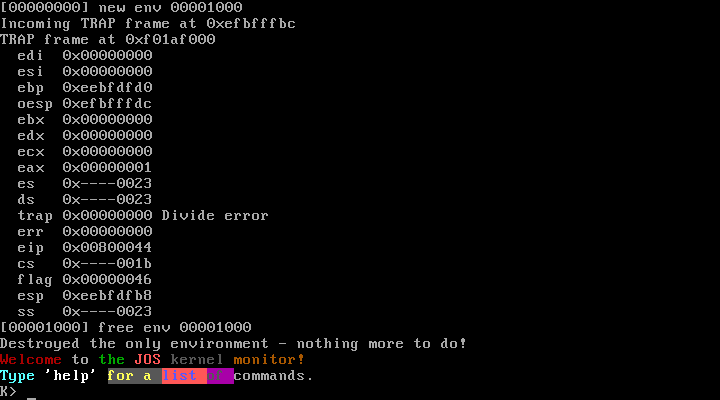
\includegraphics[scale=0.40]{/home/zhangchi/lab/report/idt_setup.png}
\end{figure}

我们来测试一下,调用评分:make grade

\begin{lstlisting}[style=console]
make[1]: Leaving directory `/home/zhangchi/lab'
sh ./grade-lab3.sh
make[1]: Entering directory `/home/zhangchi/lab'
make[1]: Nothing to be done for `all'.
make[1]: Leaving directory `/home/zhangchi/lab'
divzero: OK (1.5s)
softint: OK (1.2s)
badsegment: OK (1.2s)
Part A score: 30/30

faultread: missing '.00001000. user fault va 00000000 ip 008.....'
WRONG (1.2s)
faultreadkernel: missing '.00001000. user fault va f0100000 ip 008.....'
WRONG (1.2s)
faultwrite: missing '.00001000. user fault va 00000000 ip 008.....'
WRONG (1.2s)
faultwritekernel: missing '.00001000. user fault va f0100000 ip 008.....'
WRONG (1.2s)
breakpoint: got unexpected line '.00001000. free env 00001000'
WRONG (1.2s)
testbss: missing 'Making sure bss works right...'
missing 'Yes, good.  Now doing a wild write off the end...'
missing '.00001000. user fault va 00c..... ip 008.....'
missing '.00001000. free env 00001000'
WRONG (1.2s)
hello: missing 'hello, world'
missing 'i am environment 00001000'
missing '.00001000. exiting gracefully'
WRONG (1.2s)
buggyhello: missing '.00001000. user_mem_check assertion failure for va 00000001'
WRONG (1.2s)
buggyhello2: missing '.00001000. user_mem_check assertion failure for va 0....000'
WRONG (1.2s)
evilhello: missing '.00001000. user_mem_check assertion failure for va f0100...'
WRONG (1.2s)
Part B score: 0/50

Score: 30/80
make: *** [grade] Error 1
zhangchi@zhangchi-vostro1400:~/lab$ 
\end{lstlisting}

可以看到Part A的分数都拿到了,至此Part A就全部完成了,欢呼一下!

\vspace{4em}

\begin{lstlisting}[style=exercise]
|Questions|

Answer the following questions in your answers-lab3.txt:

1. What is the purpose of having an individual handler function for each exception/interrupt? (i.e., if all exceptions/interrupts were delivered to the same handler, what feature that exists in the current implementation could not be provided?)

2. Did you have to do anything to make the user/softint program behave correctly? The grade script expects it to produce a general protection fault (trap 13), but softint's code says int $14. Why should this produce interrupt vector 13? What happens if the kernel actually allows softint's int $14 instruction to invoke the kernel's page fault handler (which is interrupt vector 14)?
\end{lstlisting}

\begin{enumerate}
\item{现在JOS的中断处理程序在真正的处理之前要将中断号放入内核栈以组织成Trapframe的结构,但是如果所有中断都跳到同一个处理程序,那么就无法区分是哪个中断调用进来的,也就无法正确设置它们的中断号了}
\item{现在我们在中断向量里设置的14号Page fault的调用权限是0,即只能内核抛出,所以直接在softint中用int指令调用肯定产生的General Protection Fault权限错误,如下图所示:

\begin{lstlisting}[style=console]
qemu -hda obj/kern/kernel.img -serial mon:stdio
6828 decimal is 15254 octal!
Hooray! Passed all test cases for stdlib!!
Physical memory: 66556K available, base = 640K, extended = 65532K
check_page_alloc() succeeded!
page_check() succeeded!
check_boot_pgdir() succeeded!
[00000000] new env 00001000
Incoming TRAP frame at 0xefbfffbc
TRAP frame at 0xf01af000
  edi  0x00000000
  esi  0x00000000
  ebp  0xeebfdfd0
  oesp 0xefbfffdc
  ebx  0x00000000
  edx  0x00000000
  ecx  0x00000000
  eax  0x00000000
  es   0x----0023
  ds   0x----0023
  trap 0x0000000d General Protection
  err  0x00000072
  eip  0x00800037
  cs   0x----001b
  flag 0x00000046
  esp  0xeebfdfd0
  ss   0x----0023
[00001000] free env 00001000
Destroyed the only environment - nothing more to do!
Welcome to the JOS kernel monitor!
Type 'help' for a list of commands.
K> 
\end{lstlisting}

\vspace{2em}

如果将14号Page fault权限打开,即中断向量中权限设置为3给用户调用,这样可以试试,QEMU成功抛出了Page Fault:

\begin{lstlisting}[style=console, numbers=left]
qemu -hda obj/kern/kernel.img -serial mon:stdio
6828 decimal is 15254 octal!
Hooray! Passed all test cases for stdlib!!
Physical memory: 66556K available, base = 640K, extended = 65532K
check_page_alloc() succeeded!
page_check() succeeded!
check_boot_pgdir() succeeded!
[00000000] new env 00001000
Incoming TRAP frame at 0xefbfffc0
TRAP frame at 0xefbfffc0
  edi  0x00000000
  esi  0x00000000
  ebp  0xeebfdfd0
  oesp 0xefbfffe0
  ebx  0x00000000
  edx  0x00000000
  ecx  0x00000000
  eax  0x00000000
  es   0x----0023
  ds   0x----0023
  trap 0x0000000e Page Fault
  err  0x00800039
  eip  0x0000001b
  cs   0x----0046
  flag 0xeebfdfd0
  esp  0x00000023
  ss   0x----0000
[00001000] free env 00001000
Destroyed the only environment - nothing more to do!
Welcome to the JOS kernel monitor!
Type 'help' for a list of commands.
K> 
\end{lstlisting}

\highlight{\large 但是,不要高兴太早!} 

查阅中断向量的描述我们就可以知道Page fault中断是需要压入错误代码的!但是前面我们已经说过,用户用int指令调用中断是不会压入错误代码的。可是我们在kern/trapentry.S中为Page fault指定的中断处理程序默认认为系统为我们放入了错误码,所以不会补齐。那么当我们用int调用中断处理程序造成的后果是什么?\highlight{栈中没有放入错误码!!!} \\

请注意上面打印出信息的第22行关于err开始,其实就发生了错位,err是原本eip的值0x00800039(是不是很眼熟?)后面都是依次错位的。 \\

还记得前面说过内核栈的压入结构要对应Trapframe么?如果少了一个成员,我们再把这个Trapframe传到trap ()中进行处理,那么在访问Trapframe中的最后一个DWORD(也就是访问ss寄存器时),肯定就\highlight{访问到KSTACKTOP之上的空间上去了}!!那么为什么打印ss时候还可以正常打印出东西呢?\\

在inc/memlayout.h中可以看到,KSTACKTOP上的空间为VPT,即系统页目录。如果以VPT的虚拟地址来访问内存,VPT的PDX会找到系统页目录,PTX为0,会找到页目录中第0个页表的物理地址,然后OFFSET为0,访问的是第0个页表的第0个页表项。因为我们知道,JOS在载入softint时会分配物理页放入elf文件,我们可以查看一下user/user.ld中关于文件中stab节的链接地址

\begin{lstlisting}[style=ccode, language=make, firstnumber=39, title={\scriptsize \ttfamily \bfseries user/user.ld}]
    /* Place debugging symbols so that they can be found by
     * the kernel debugger.
     * Specifically, the four words at 0x200000 mark the beginning of
     * the stabs, the end of the stabs, the beginning of the stabs
     * string table, and the end of the stabs string table, respectively.
     */

    .stab_info 0x200000 : {
        LONG(__STAB_BEGIN__);
        LONG(__STAB_END__);
        LONG(__STABSTR_BEGIN__);
        LONG(__STABSTR_END__);
    }

    .stab : {
        __STAB_BEGIN__ = DEFINED(__STAB_BEGIN__) ? __STAB_BEGIN__ : .;
        *(.stab);
        __STAB_END__ = DEFINED(__STAB_END__) ? __STAB_END__ : .;
        BYTE(0)        /* Force the linker to allocate space
                   for this section */
    }

    .stabstr : {
        __STABSTR_BEGIN__ = DEFINED(__STABSTR_BEGIN__) ? __STABSTR_BEGIN__ : .;
        *(.stabstr);
        __STABSTR_END__ = DEFINED(__STABSTR_END__) ? __STABSTR_END__ : .;
        BYTE(0)        /* Force the linker to allocate space
                   for this section */
    }

    /DISCARD/ : {
        *(.eh_frame .note.GNU-stack .comment)
    }
\end{lstlisting}

可以看到这个调试信息被映射到了0x200000地址,实际上这段信息就是我们刚才在越过KSTACKTOP后访问到的信息,如果我们尝试在user/user.ld中删除这段,重新编译运行JOS的话,会看到:

\begin{lstlisting}[style=console]
qemu -nographic -hda obj/kern/kernel.img -serial mon:stdio
6828 decimal is 15254 octal!
Hooray! Passed all test cases for stdlib!!
Physical memory: 66556K available, base = 640K, extended = 65532K
check_page_alloc() succeeded!
page_check() succeeded!
check_boot_pgdir() succeeded!
[00000000] new env 00001000
Incoming TRAP frame at 0xefbfffc0
TRAP frame at 0xefbfffc0
  edi  0x00000000
  esi  0x00000000
  ebp  0xeebfdfd0
  oesp 0xefbfffe0
  ebx  0x00000000
  edx  0x00000000
  ecx  0x00000000
  eax  0x00000000
  es   0x----0023
  ds   0x----0023
  trap 0x0000000e Page Fault
  err  0x00800039
  eip  0x0000001b
  cs   0x----0046
  flag 0xeebfdfd0
  esp  0x00000023
Incoming TRAP frame at 0xefbfff30
TRAP frame at 0xefbfff30
  edi  0x00000000
  esi  0xefbfffc0
  ebp  0xefbfff84
  oesp 0xefbfff50
  ebx  0xefbfffc0
  edx  0x000003d5
  ecx  0x000003d5
  eax  0x00000000
  es   0x----0010
  ds   0x----0010
  trap 0x0000000e Page Fault
  err  0x00000000
  eip  0xf0103c4f
  cs   0x----0008
  flag 0x00000092
  esp  0xf0106bba
  ss   0x----0023
kernel panic at kern/trap.c:174: unhandled trap in kernel
Welcome to the JOS kernel monitor!
Type 'help' for a list of commands.
K> 

\end{lstlisting}

可以看到,在第一个Page fault处理程序中(由softint中使用int指令调用),在打印最后一个ss时,又发生了Page fault中断(由系统产生),因为去掉softint的stab节映射以后,\highlight{VPT上就没有相应的映射页了},这样就发生了第二次Page fault了。


\highlight{\Huge 谢谢实验室的张顺廷师兄的热心指导!!!!}

}
\end{enumerate}





\section{Page Faults, Breakpoints Exceptions, and System Calls}

\subsection{Handling Page Faults}

\begin{lstlisting}[style=exercise]
|Exercise 5|. Modify trap_dispatch() to dispatch page fault exceptions to page_fault_handler(). You should now be able to get make grade to succeed on the faultread, faultreadkernel, faultwrite, and faultwritekernel tests. If any of them don't work, figure out why and fix them. Remember that you can boot JOS into a particular user program using make run-x or make run-x-nox.
\end{lstlisting}

加一句话就好:

\begin{lstlisting}[style=ccode, title={\scriptsize \ttfamily \bfseries kern/trap.c: trap\_dispatch()}]
static void
trap_dispatch(struct Trapframe *tf)
{
    if (tf->tf_trapno == T_PGFLT) 
        page_fault_handler (tf);
        
    // Unexpected trap: The user process or the kernel has a bug.
    print_trapframe(tf);
\end{lstlisting}


\subsection{The Breakpoint Exception}

\begin{lstlisting}[style=exercise]
|Exercise 6|. Modify trap_dispatch() to make breakpoint exceptions invoke the kernel monitor. You should now be able to get make grade to succeed on the breakpoint test.
\end{lstlisting}

同样加一句话就好:

\begin{lstlisting}[style=ccode, title={\scriptsize \ttfamily \bfseries kern/trap.c: trap\_dispatch()}]
static void
trap_dispatch(struct Trapframe *tf)
{
    if (tf->tf_trapno == T_PGFLT) 
        page_fault_handler (tf);

    if (tf->tf_trapno == T_BRKPT)
        monitor (tf);
\end{lstlisting}

\vspace{4em}

\begin{lstlisting}[style=exercise]
|Questions|

1. The break point test case will either generate a break point exception or a general protection fault depending on how you initialized the break point entry in the IDT (i.e., your call to SETGATE from idt_init). Why? How did you need to set it in order to get the breakpoint exception to work as specified above?

2. What do you think is the point of these mechanisms, particularly in light of what the user/softint test program does?
\end{lstlisting}

\begin{enumerate}
\item{权限问题,在\funcname{idt\_init()} 中已经说明过了}
\item{关于softint的执行过程也已经说明过了}
\end{enumerate}

\subsection{System calls}


\begin{lstlisting}[style=exercise]
|Exercise 7|. Add a handler in the kernel for interrupt vector T_SYSCALL. You will have to edit kern/trapentry.S and kern/trap.c's idt_init(). You also need to change trap_dispatch() to handle the system call interrupt by calling syscall() (defined in kern/syscall.c) with the appropriate arguments, and then arranging for the return value to be passed back to the user process in %eax. Finally, you need to implement syscall() in kern/syscall.c. Make sure syscall() returns -E_INVAL if the system call number is invalid. You should read and understand lib/syscall.c (especially the inline assembly routine) in order to confirm your understanding of the system call interface. You may also find it helpful to read inc/syscall.h.

Run the user/hello program under your kernel (make run-hello). It should print "hello, world" on the console and then cause a page fault in user mode. If this does not happen, it probably means your system call handler isn't quite right. You should also now be able to get make grade to succeed on the testbss test.
\end{lstlisting}

这个Exercise让我们可以开始处理系统中断,根据提示,首先修改kern/trap.c中的\funcname{idt\_init()}以及kern/trapentry.S添加相应的中断服务程序和中断向量,然后修改kern/trap.c

\begin{lstlisting}[style=ccode, title={\scriptsize \ttfamily \bfseries kern/trap.c: trap\_dispatch()}]
    if (tf->tf_trapno == T_PGFLT) 
        page_fault_handler (tf);

    if (tf->tf_trapno == T_BRKPT)
        monitor (tf);

    int r;

    if (tf->tf_trapno == T_SYSCALL) {
        
        r = syscall (
                tf->tf_regs.reg_eax, 
                tf->tf_regs.reg_edx, 
                tf->tf_regs.reg_ecx, 
                tf->tf_regs.reg_ebx, 
                tf->tf_regs.reg_edi, 
                tf->tf_regs.reg_esi); 
        if (r < 0)
            panic ("trap_dispatch: The System Call number is invalid");

        tf->tf_regs.reg_eax = r;

        return;
    }
\end{lstlisting}

然后接着完成kern/syscall.c

\begin{lstlisting}[style=ccode, title={\scriptsize \ttfamily \bfseries kern/syscall.c: syscall()}]
// Dispatches to the correct kernel function, passing the arguments.
int32_t
syscall(uint32_t syscallno, uint32_t a1, uint32_t a2, uint32_t a3, uint32_t a4, uint32_t a5)
{
    int32_t r = 0;

    switch (syscallno) {
        case SYS_cputs: 
            sys_cputs ((const char*) a1, (size_t)a2); break;              
        case SYS_cgetc: 
            r = sys_cgetc (); break;
        case SYS_getenvid:
            r = sys_getenvid (); break;
        case SYS_env_destroy:
            r = sys_env_destroy ((envid_t) a1); break;
        default:
            r = -E_INVAL;
    }
   
    return r;

    panic("syscall not implemented");
}

\end{lstlisting}

然后运行测试可以通过testbss测试。没有什么值得注意的地方,按照提示一步一步写就好了

\subsection{User-mode startup}

\begin{lstlisting}[style=exercise]
|Exercise 8|. Add the required code to the user library, then boot your kernel. You should see user/hello print "hello, world" and then print "i am environment 00000800". user/hello then attempts to "exit" by calling sys_env_destroy() (see lib/libmain.c and lib/exit.c). Since the kernel currently only supports one user environment, it should report that it has destroyed the only environment and then drop into the kernel monitor. You should be able to get make grade to succeed on the hello test.
\end{lstlisting}

改一句话即可:

\begin{lstlisting}[style=ccode, title={\scriptsize \ttfamily \bfseries lib/libmain.c: libmain()}]
void
libmain(int argc, char **argv)
{
	// set env to point at our env structure in envs[].
	// LAB 3: Your code here.
	env = envs + ENVX(sys_getenvid ());
\end{lstlisting}

其中\funcname{sys\_getenvid()} 是lib中包装好的函数,在其内部是使用调用系统中断实现的。这个时候在运行make run-hello,可以看到已经正常运行了:

\begin{lstlisting}[style=console]
qemu -hda obj/kern/kernel.img -serial mon:stdio
6828 decimal is 15254 octal!
Hooray! Passed all test cases for stdlib!!
Physical memory: 66556K available, base = 640K, extended = 65532K
check_page_alloc() succeeded!
page_check() succeeded!
check_boot_pgdir() succeeded!
[00000000] new env 00001000
Incoming TRAP frame at 0xefbfffbc
Incoming TRAP frame at 0xefbfffbc
hello, world
Incoming TRAP frame at 0xefbfffbc
i am environment 00001000
Incoming TRAP frame at 0xefbfffbc
[00001000] exiting gracefully
[00001000] free env 00001000
Destroyed the only environment - nothing more to do!
Welcome to the JOS kernel monitor!
Type 'help' for a list of commands.
K> 

\end{lstlisting}

\subsection{Page faults and memory protection}

\begin{lstlisting}[style=exercise]
|Exercise 9|. Change kern/trap.c to panic if a page fault happens in kernel mode.

Hint: to determine whether a fault happened in user mode or in kernel mode, check the low bits of the tf_cs.

Read user_mem_assert in kern/pmap.c and implement user_mem_check in that same file.

Change kern/syscall.c to sanity check arguments to system calls.

Boot your kernel, running user/buggyhello. The environment should be destroyed, and the kernel should not panic. You should see:

	[00001000] user_mem_check assertion failure for va 00000001
	[00001000] free env 00001000
	Destroyed the only environment - nothing more to do!
	
Finally, change debuginfo_eip in kern/kdebug.c to call user_mem_check on usd, stabs, and stabstr. If you now run user/breakpoint, you should be able to run backtrace from the kernel monitor and see the backtrace traverse into lib/libmain.c before the kernel panics with a page fault. What causes this page fault? You don't need to fix it, but you should understand why it happens.
\end{lstlisting}

照着直接改代码,没有啥好注意的,我直接贴代码了。

首先是在 \funcname{ page\_fault\_handler() } 中处理内核态中抛出页面错误:

\begin{lstlisting}[style=ccode, title={\scriptsize \ttfamily \bfseries kern/trap.c: page\_fault\_handler()}]
void
page_fault_handler(struct Trapframe *tf)
{
	uint32_t fault_va;

	// Read processor's CR2 register to find the faulting address
	fault_va = rcr2();

	// Handle kernel-mode page faults.
        if ((tf->tf_cs & 3) == 0)
            panic ("kernel-mode page faults");
 
	// We've already handled kernel-mode exceptions, so if we get here,
	// the page fault happened in user mode.

	// Destroy the environment that caused the fault.
	cprintf("[%08x] user fault va %08x ip %08x\n",
		curenv->env_id, fault_va, tf->tf_eip);
	print_trapframe(tf);
	env_destroy(curenv);
}
\end{lstlisting}

然后是检测线性地址的页面是否有效:

\begin{lstlisting}[style=ccode, title={\scriptsize \ttfamily \bfseries kern/pmap.c: user\_mem\_check()}]
int
user_mem_check(struct Env *env, const void *va, size_t len, int perm)
{
	// LAB 3: Your code here. 
    
    uintptr_t lva = (uintptr_t) va;
    uintptr_t rva = (uintptr_t) va + len - 1;

    perm = perm|PTE_U|PTE_P;

    pte_t *pte;
    uintptr_t idx_va;

    for (idx_va = lva; idx_va <= rva; idx_va += PGSIZE) {

        if (idx_va >= ULIM) {
            user_mem_check_addr = idx_va;
            return -E_FAULT;
        }

        pte = pgdir_walk (env->env_pgdir, (void*)idx_va, 0);

        if (pte == NULL || (*pte & perm) != perm) {  
            user_mem_check_addr = idx_va;
            return -E_FAULT;
        }

        idx_va = ROUNDDOWN (idx_va, PGSIZE);
    }

    return 0;
}
\end{lstlisting}

然后在\funcname{sys\_cputs()}中加入相应对用户空间地址的检查:

\begin{lstlisting}[style=ccode, title={\scriptsize \ttfamily \bfseries kern/syscall.c: sys\_cputs()}]
static void
sys_cputs(const char *s, size_t len)
{
	// Check that the user has permission to read memory [s, s+len).
	// Destroy the environment if not.
	
	// LAB 3: Your code here.
        user_mem_assert (curenv, s, len, PTE_U);

	// Print the string supplied by the user.
	cprintf("%.*s", len, s);
}
\end{lstlisting}

做到这里,我们运行user/buggyhello已经可以得到正确的结果。接下来再改一下kern/kdebug.c中完成对stab的检查就大功告成了!

\begin{lstlisting}[style=ccode, title={\scriptsize \ttfamily \bfseries kern/kdebug.c: debuginfo\_eip()}]
	// Make sure this memory is valid.
	// Return -1 if it is not.  Hint: Call user_mem_check.
	// LAB 3: Your code here.
        
        if (user_mem_check (curenv, usd, sizeof (struct UserStabData), PTE_U) < 0)
            return -1;

	stabs = usd->stabs;
	stab_end = usd->stab_end;
	stabstr = usd->stabstr;
	stabstr_end = usd->stabstr_end;

	// Make sure the STABS and string table memory is valid.
	// LAB 3: Your code here.

        if (user_mem_check (curenv, stabs, stab_end - stabs, PTE_U) < 0
        || user_mem_check (curenv, stabstr, stabstr_end - stabstr, PTE_U) < 0) 
            return -1;
\end{lstlisting}

启动make run-breakpoint,使用backtrace命令页面溢出了:

\begin{lstlisting}[style=console]
qemu -hda obj/kern/kernel.img -serial mon:stdio
6828 decimal is 15254 octal!
Hooray! Passed all test cases for stdlib!!
Physical memory: 66556K available, base = 640K, extended = 65532K
check_page_alloc() succeeded!
page_check() succeeded!
check_boot_pgdir() succeeded!
[00000000] new env 00001000
Incoming TRAP frame at 0xefbfffbc
Incoming TRAP frame at 0xefbfffbc
Welcome to the JOS kernel monitor!
Type 'help' for a list of commands.
TRAP frame at 0xf01b0000
  edi  0x00000000
  esi  0x00000000
  ebp  0xeebfdfd0
  oesp 0xefbfffdc
  ebx  0x00000000
  edx  0x00000000
  ecx  0x00000000
  eax  0xeec00000
  es   0x----0023
  ds   0x----0023
  trap 0x00000003 Breakpoint
  err  0x00000000
  eip  0x00800038
  cs   0x----001b
  flag 0x00000046
  esp  0xeebfdfd0
  ss   0x----0023
K> backtrace
Stack backtrace:
  ebp efbfff10  eip f01008ea  args 00000001 efbfff28 f01b0000 00000000 f017d960
         kern/monitor.c:419: monitor+274
  ebp efbfff80  eip f0103e54  args f01b0000 efbfffbc 00000000 00000000 00000000
         kern/trap.c:174: trap+71
  ebp efbfffb0  eip f0103f9e  args efbfffbc 00000000 00000000 eebfdfd0 efbfffdc
         kern/trapentry.S:83: <unknown>+0
  ebp eebfdfd0  eip 0080007c  args 00000000 00000000 00000000 00000000 00000000
         lib/libmain.c:26: libmain+64
Incoming TRAP frame at 0xefbffe6c
kernel panic at kern/trap.c:249: kernel-mode page faults
Welcome to the JOS kernel monitor!
Type 'help' for a list of commands.
K> 
\end{lstlisting}

通过跟踪发现是访问libmain外层的函数,从ebp中取出eip时页面错误了,这个我懒得查栈结构了。

\vspace{2em}

\begin{lstlisting}[style=exercise]
|Exercise 10|. Boot your kernel, running user/evilhello. The environment should be destroyed, and the kernel should not panic. You should see:

	[00000000] new env 00001000
	[00001000] user_mem_check assertion failure for va f0100020
	[00001000] free env 00001000
\end{lstlisting}

我们可以看看user/evilhello

\begin{lstlisting}[style=ccode, title={\scriptsize \ttfamily \bfseries user/evilhello.c}]
#include <inc/lib.h>

void
umain(void)
{
	// try to print the kernel entry point as a string!  mua ha ha!
	sys_cputs((char*)0xf010000c, 100);
}
\end{lstlisting}

我的输出结果和它的地址不太一样,应该是一访问内核第一个入口地址就出错了阿,不太清楚,这个是我的输出结果:

\begin{lstlisting}[style=console]
qemu -hda obj/kern/kernel.img -serial mon:stdio
6828 decimal is 15254 octal!
Hooray! Passed all test cases for stdlib!!
Physical memory: 66556K available, base = 640K, extended = 65532K
check_page_alloc() succeeded!
page_check() succeeded!
check_boot_pgdir() succeeded!
[00000000] new env 00001000
Incoming TRAP frame at 0xefbfffbc
Incoming TRAP frame at 0xefbfffbc
[00001000] user_mem_check assertion failure for va f010000c
[00001000] free env 00001000
Destroyed the only environment - nothing more to do!
Welcome to the JOS kernel monitor!
Type 'help' for a list of commands.
K> 
\end{lstlisting}

\vspace{4em}

因为这个星期所有的课程都开始催期中论文和作业,还有期中考试。时间实在是不够用了,所以这次一个Challenge都没做,感觉很可惜

\clearpage

\end{CJK*}
\end{document}
	

e